\documentclass{standalone}
\usepackage{tikzducks}
\usepackage{fontawesome}

\definecolor{unigold}{RGB}{203,157,52}%
\definecolor{uniblue}{RGB}{46,114,167}%
\definecolor{unired}{RGB}{177,49,34}%

\definecolor{skink}{RGB}{245,206,193}%
\definecolor{skins}{RGB}{255,222,151}%
\definecolor{skinu}{RGB}{146,113,96}%

\newcommand*{\insignia}{\node[rotate=15] at (wing) {\color{yellow!80!brown}\faLocationArrow};}
\pagecolor{gray!20!white}
\begin{document}
	
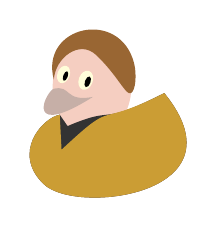
\begin{tikzpicture}
	\duck[
		tshirt=black!60!gray, 
		jacket=unigold, 
		body=skink, 
		shorthair=brown!80!black, 
		bill=skink!60!gray
	]
	\insignia
\end{tikzpicture}


\begin{tikzpicture}
	\duck[
		tshirt=black!60!gray, 
		jacket=uniblue, 
		body=skins, 
		mullet=black!60!brown, 
		bill=skins!60!gray
	]
	\fill[skins,rotate=175, xshift=-46, yshift=-74] (0.45,1.20) -- (0.50,0.80) -- (0.65,1.20);
	\fill[black!60!brown, rounded corners=1, rotate=70] (1.85,0.13) rectangle (1.91,-0.05);
	\fill[black!60!brown, rounded corners=1, rotate=90] (1.7,-0.75) rectangle (1.76,-0.97);
	\insignia
\end{tikzpicture}

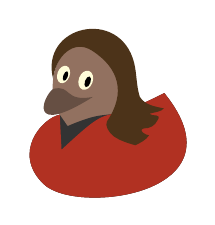
\begin{tikzpicture}
	\duck[
		tshirt=black!60!gray, 
		jacket=unired, 
		body=skinu, 
		longhair=black!60!brown, 
		bill=skinu!70!black
	]
	\insignia
\end{tikzpicture}
	
\end{document}